% Appendix A

\chapter{Figures} % Main appendix title

\label{Figures} % For referencing this appendix elsewhere, use \ref{AppendixA}

%%%%% Introduction %%%%%

\begin{figure}[th]
\centering
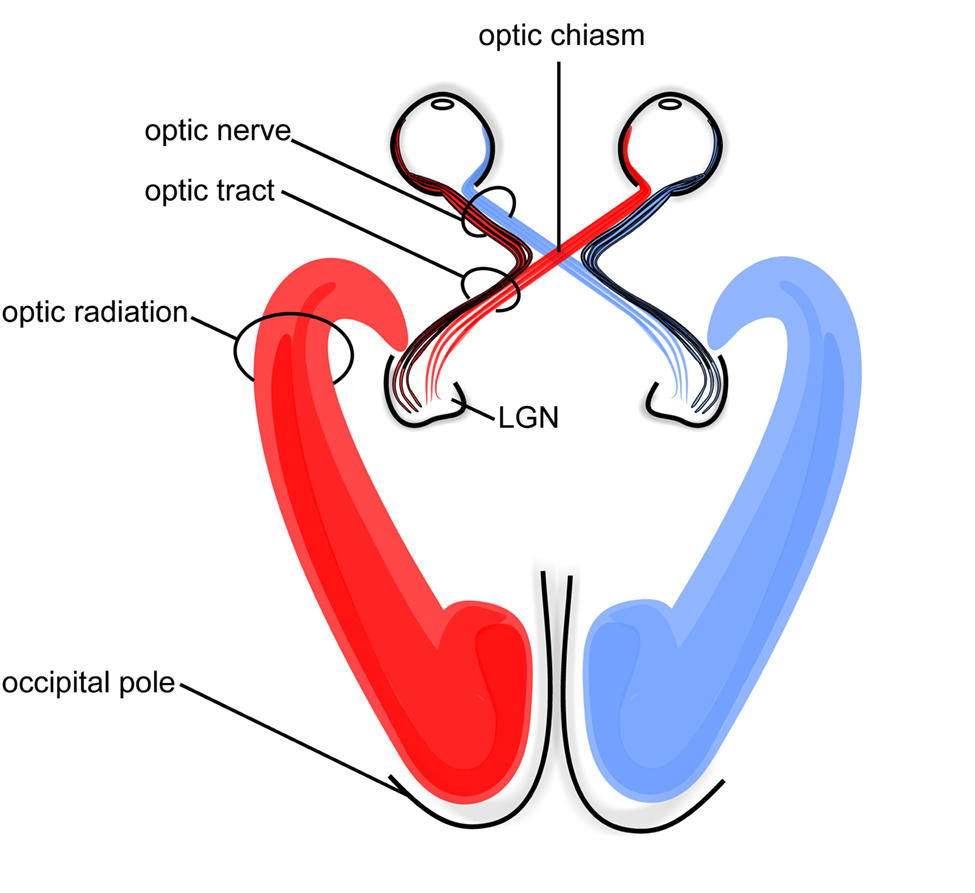
\includegraphics{Figures/visual_system}
\decoRule %puts an aesthetic horizontal line below the image
\caption[Figure]{Schéma des voies visuelles précorticales humaines (adapté de Hofer S. et al., 2010 via Wikimedia Commons [CC BY 3.0])}
\label{fig:visual_system}
\end{figure}

\begin{figure}[th]
\centering
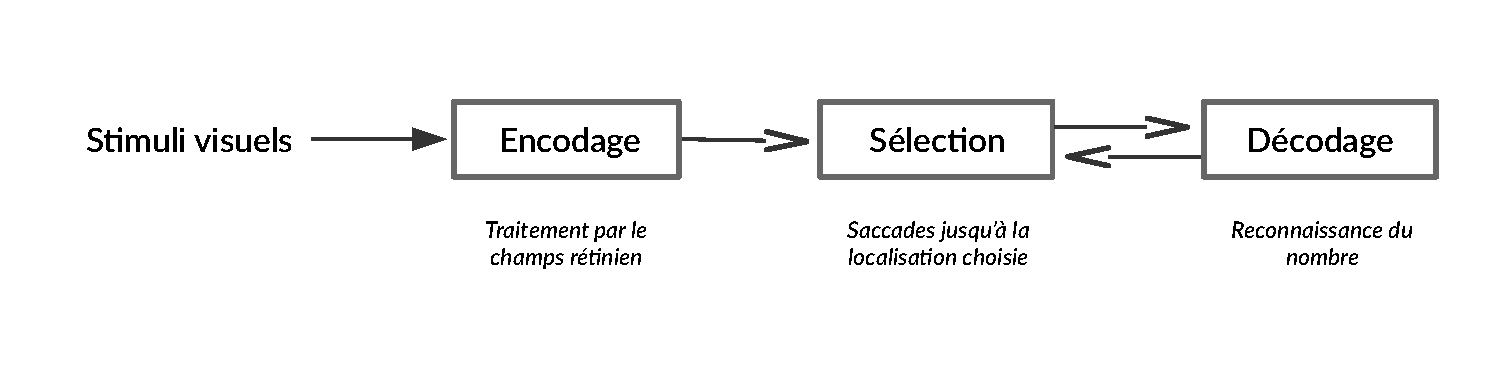
\includegraphics[scale=0.75]{Figures/visual_system_simple}
\decoRule %puts an aesthetic horizontal line below the image
\caption[Figure]{Schéma simplifié du fonctionnement du système visuel avec son \textit{équivalence dans le modèle} (adapté de \cite{Zhaoping2014})}
\label{fig:visual_system_simple}
\end{figure}

%%%%% Matériel et méthodes %%%%%

\begin{table}
\resizebox{19cm}{!}{
\begin{tabular}{| p{4cm} || l | l | p{5cm} | l | l |}
\hline
& Identifiant & Système d'explotation & Processeur & Mémoire vive & Carte graphique\\ \hline
Machine physique & ASUS ROG G75VW & Windows 7 64-bit SP1 & Intel Core I7-3610QM 2,30GHz (8CPU) &  
8 GB (DDR3) & NVIDIA GeForce GTX670M\\ \hline
Machine virtuelle (ressources allouées) & VirtualBox v.5.2.6 & Ubuntu 16.04 & 4 CPU, 90\% des ressources & 
5298 Mo & Support GPU non-utilisé\\ \hline
\end{tabular}
}
\caption[Tableau]{Matériel physique et numérique utilisé pour réaliser les modélisations}
\label{tab:materiel}
\end{table}

\begin{figure}[th]
\centering
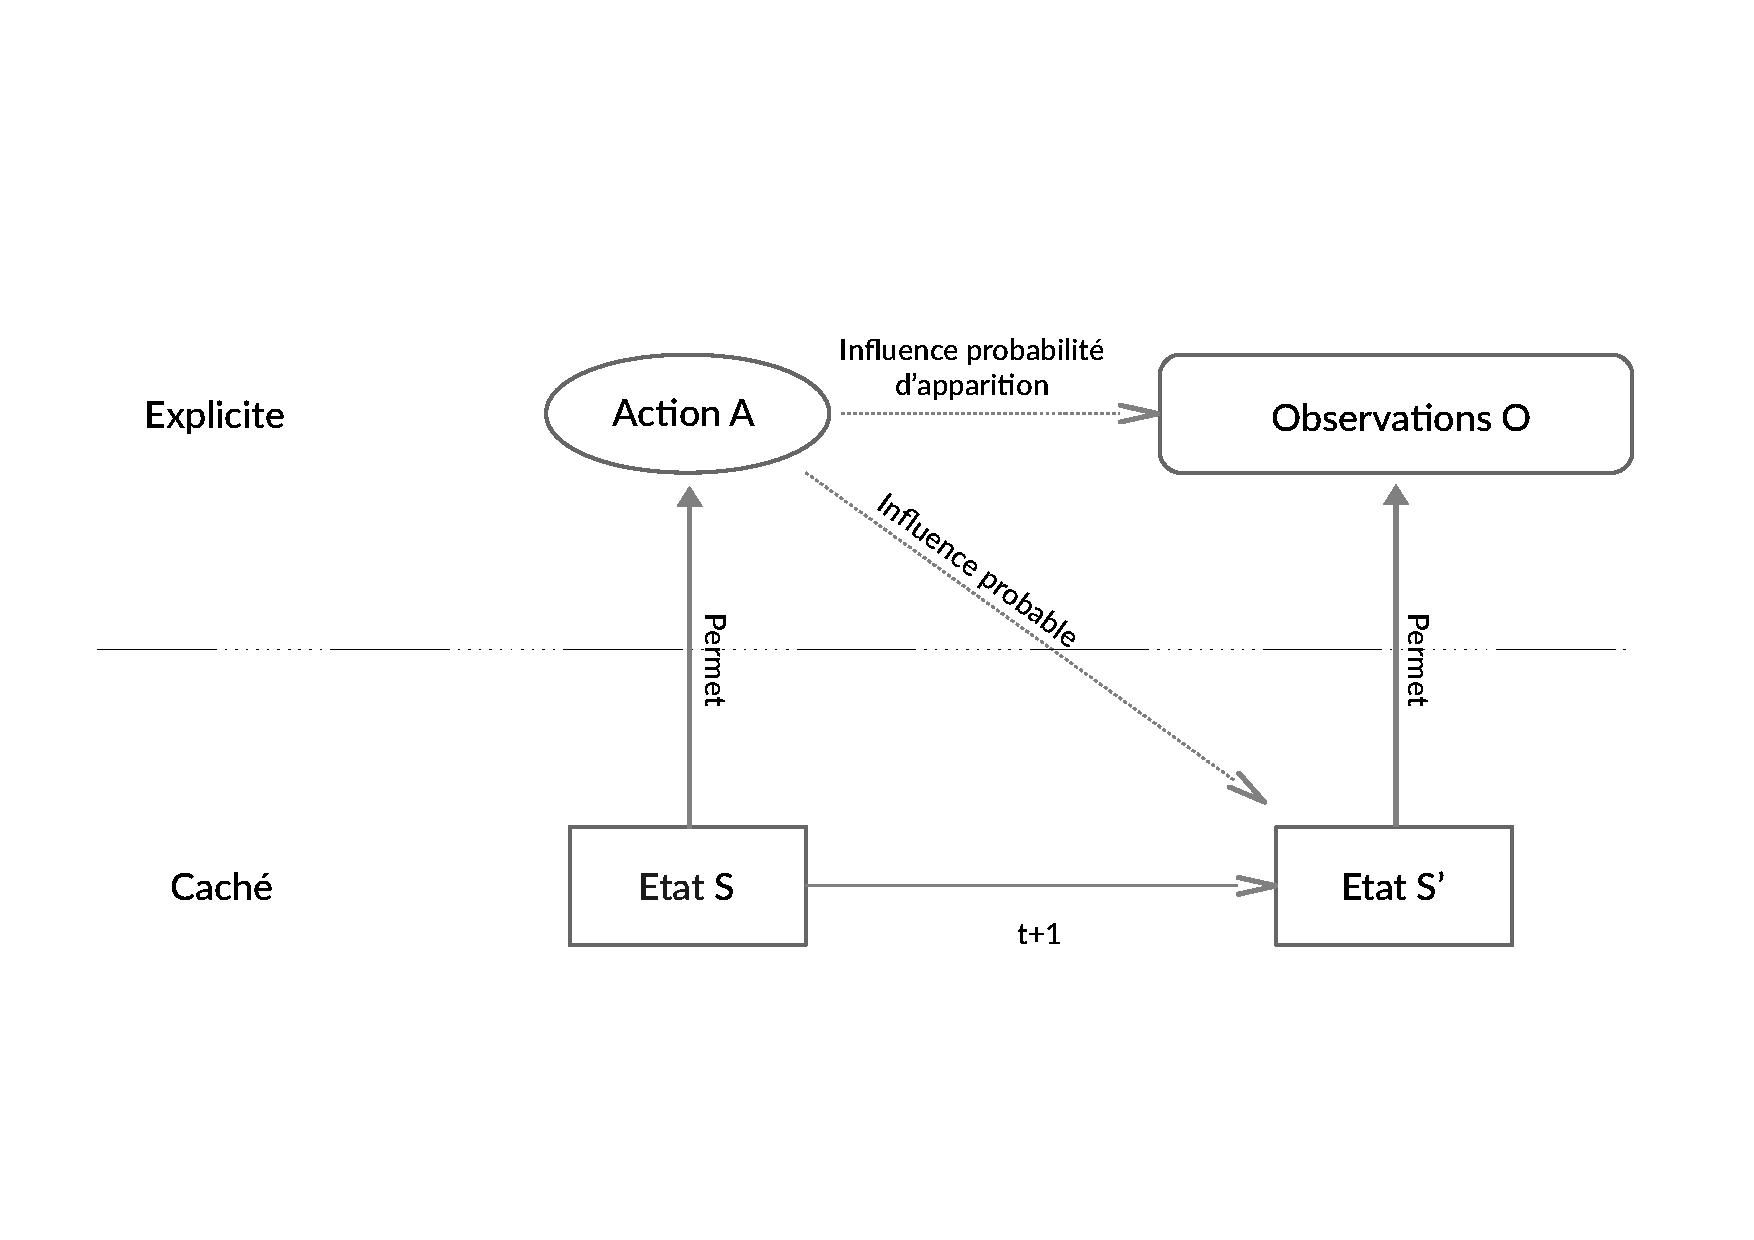
\includegraphics[scale=0.45]{Figures/POMDP}
\decoRule %puts an aesthetic horizontal line below the image
\caption[Figure]{Schéma des interations entre l'agent et son environnement au cours du temps dans un modèle POMDP}
\label{fig:POMDP}
\end{figure}

\begin{figure}[th]
\centering
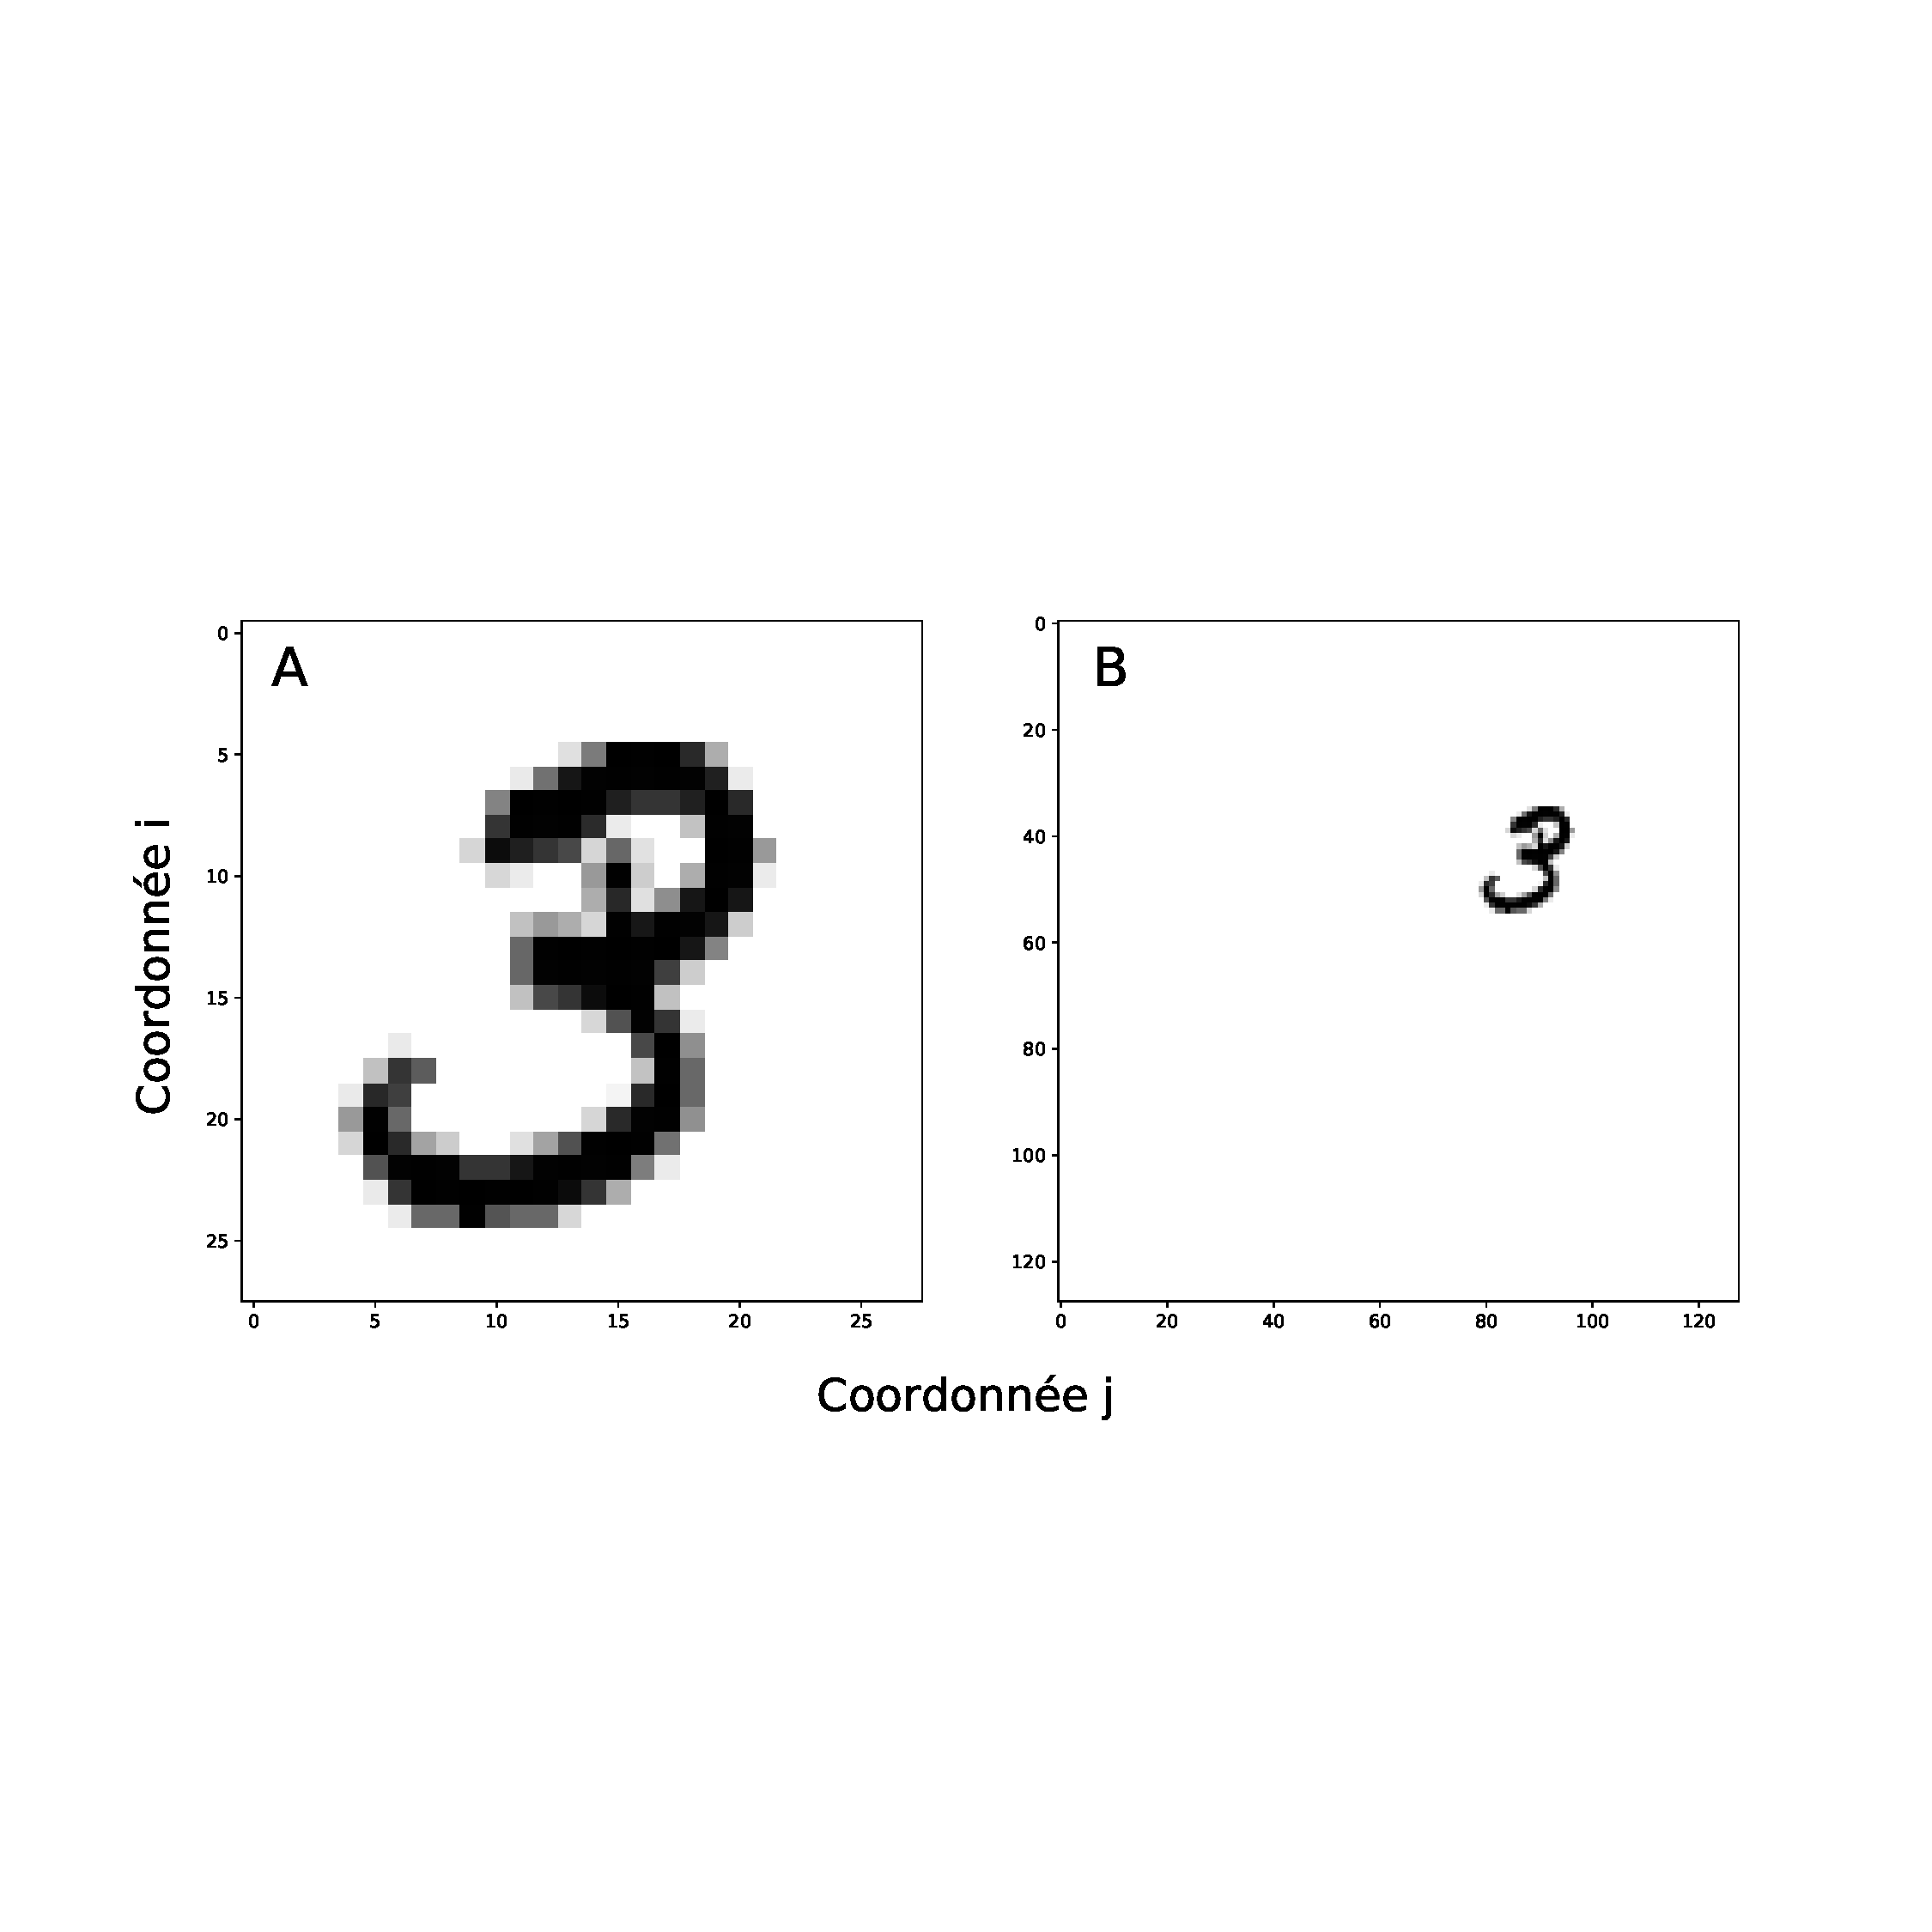
\includegraphics[scale=0.3]{Figures/mnist_reshape}
\decoRule %puts an aesthetic horizontal line below the image
\caption[Figure]{\textbf{A.} Image originale tirée de MNIST ; \textbf{B.} Image après transformation géométrique et placé aux coordonnées $(i=-20,j=25)$}
\label{fig:mnist_reshape}
\end{figure}

\begin{figure}[th]
\centering
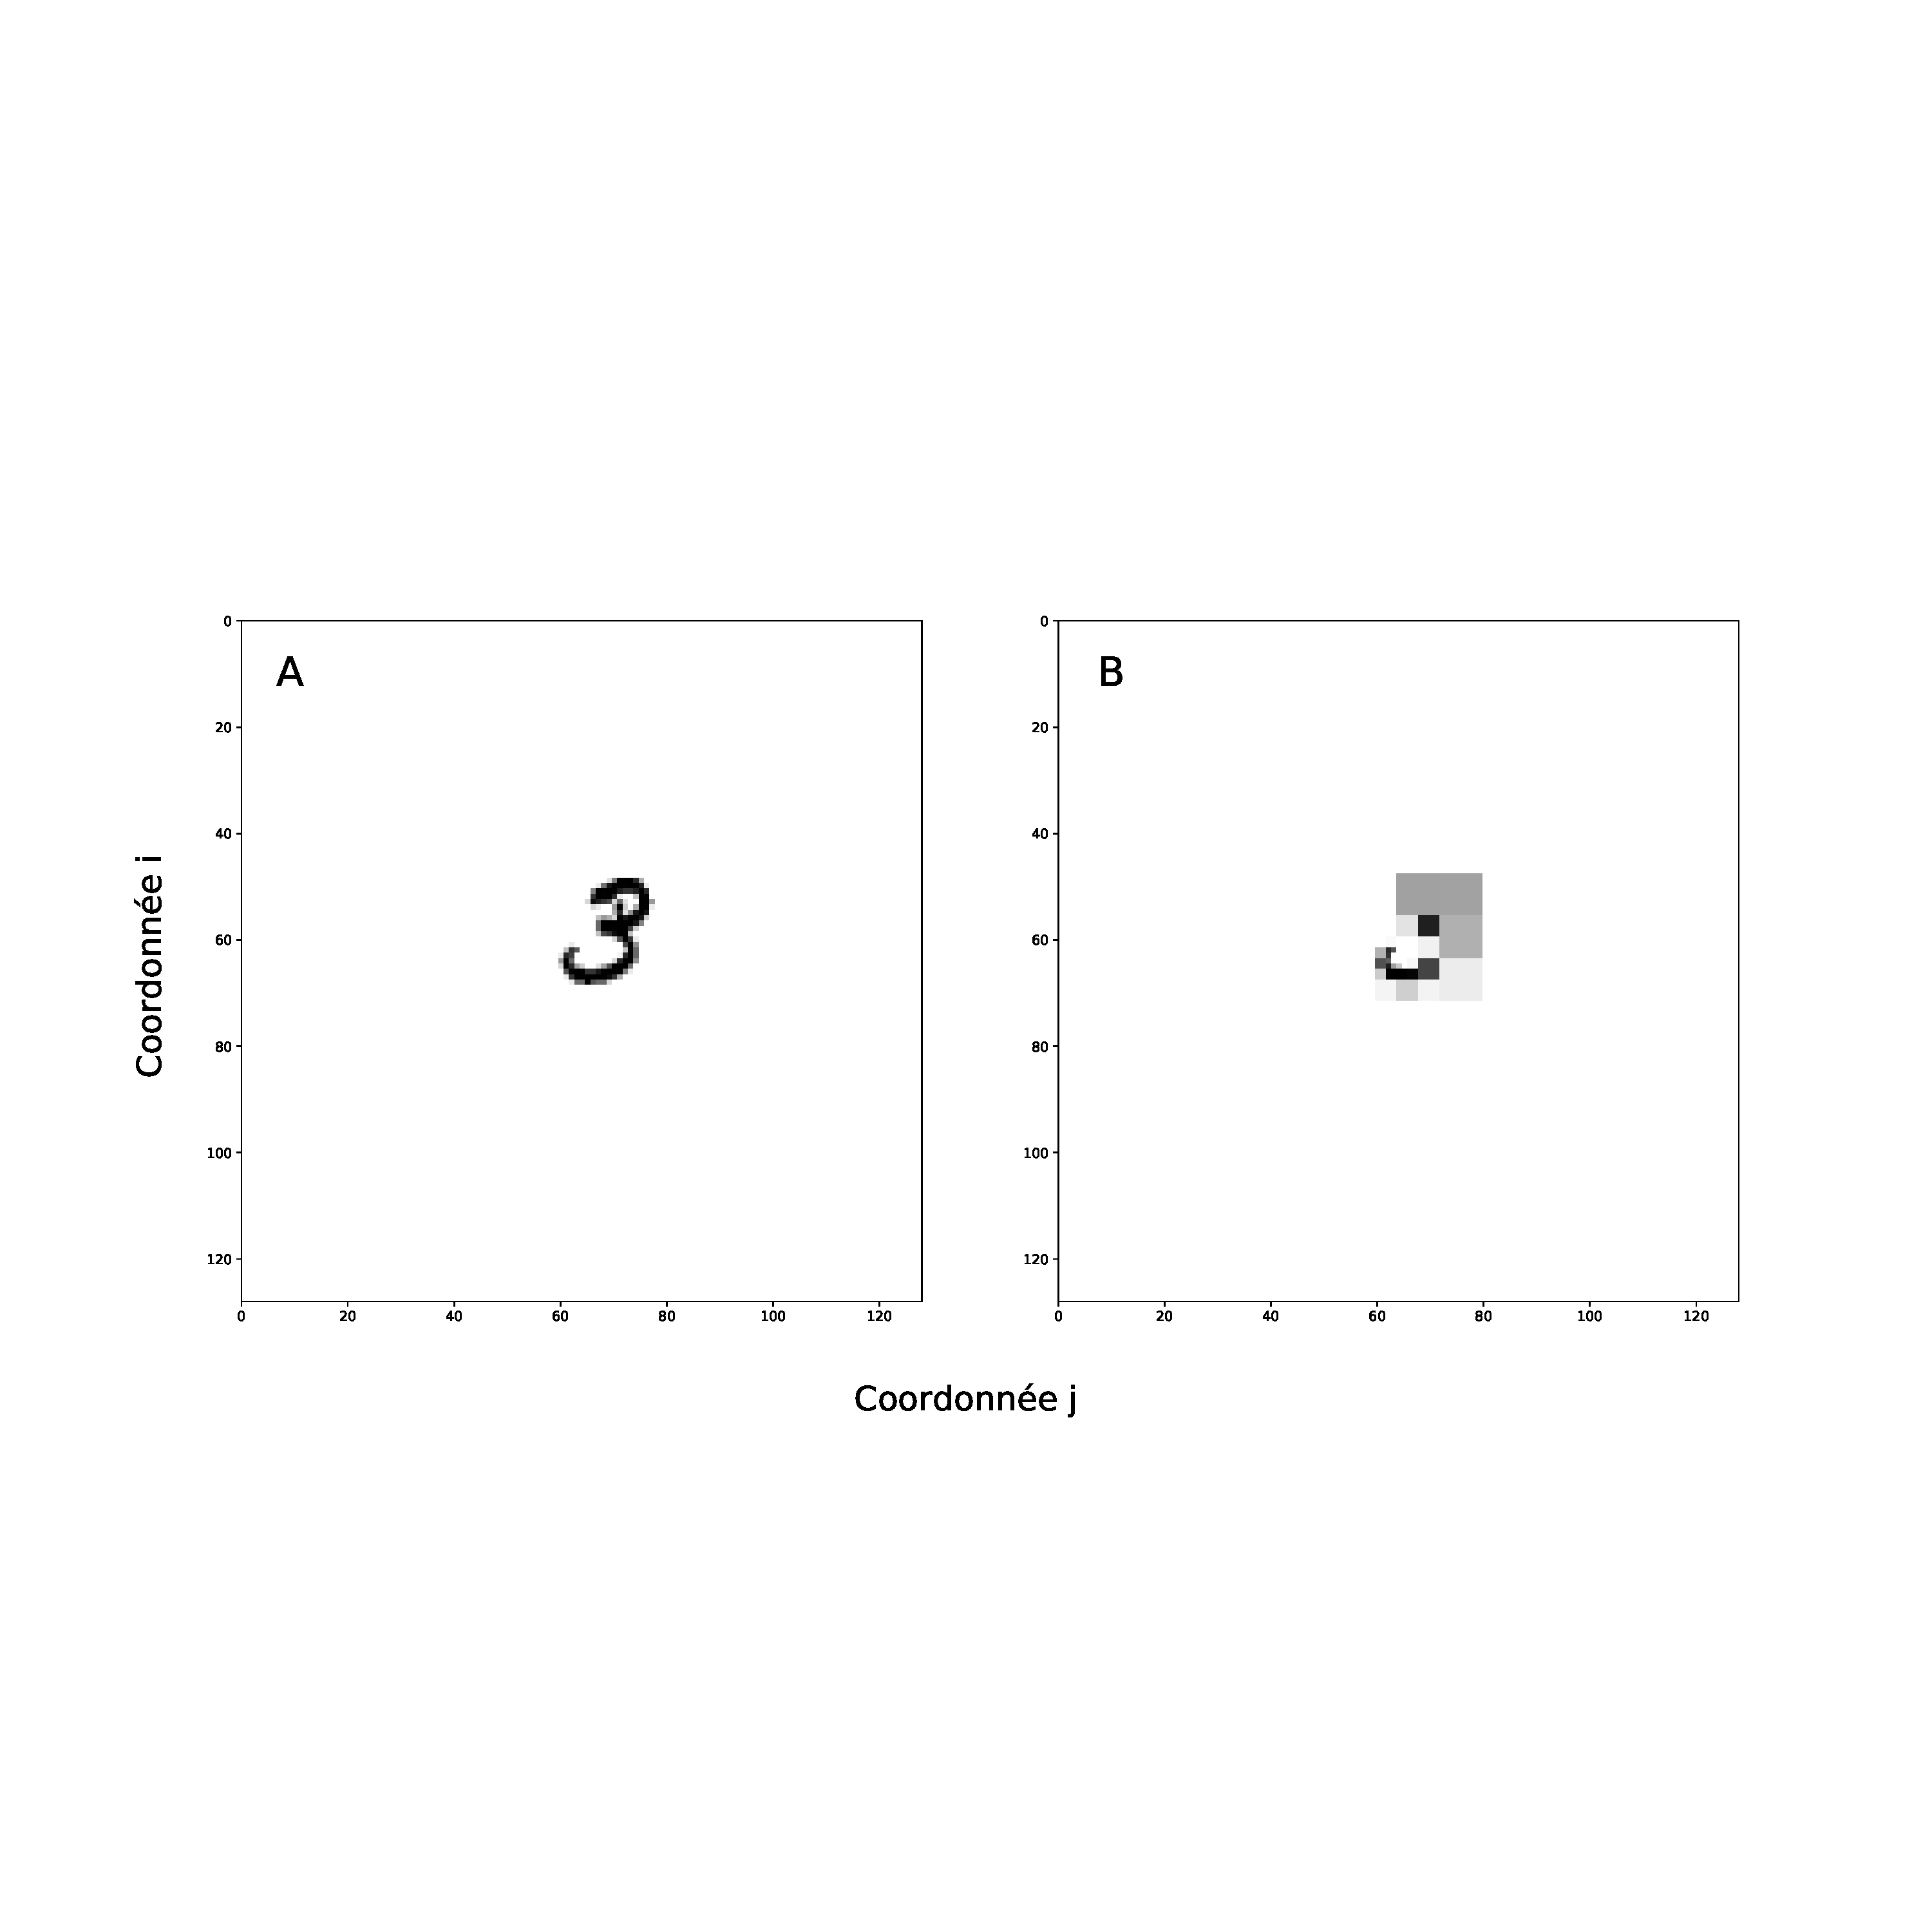
\includegraphics[scale=0.25]{Figures/wavelet_effect}
\decoRule %puts an aesthetic horizontal line below the image
\caption[Figure]{\textbf{A.} Image avant application d'un filtre et placé aux coordonnées $(i=-6,j=6)$ ; \textbf{B.} Image après transformation par le filtre \textit{Wavelets}}
\label{fig:Wavelet_effect}
\end{figure}

\begin{figure}[th]
\centering
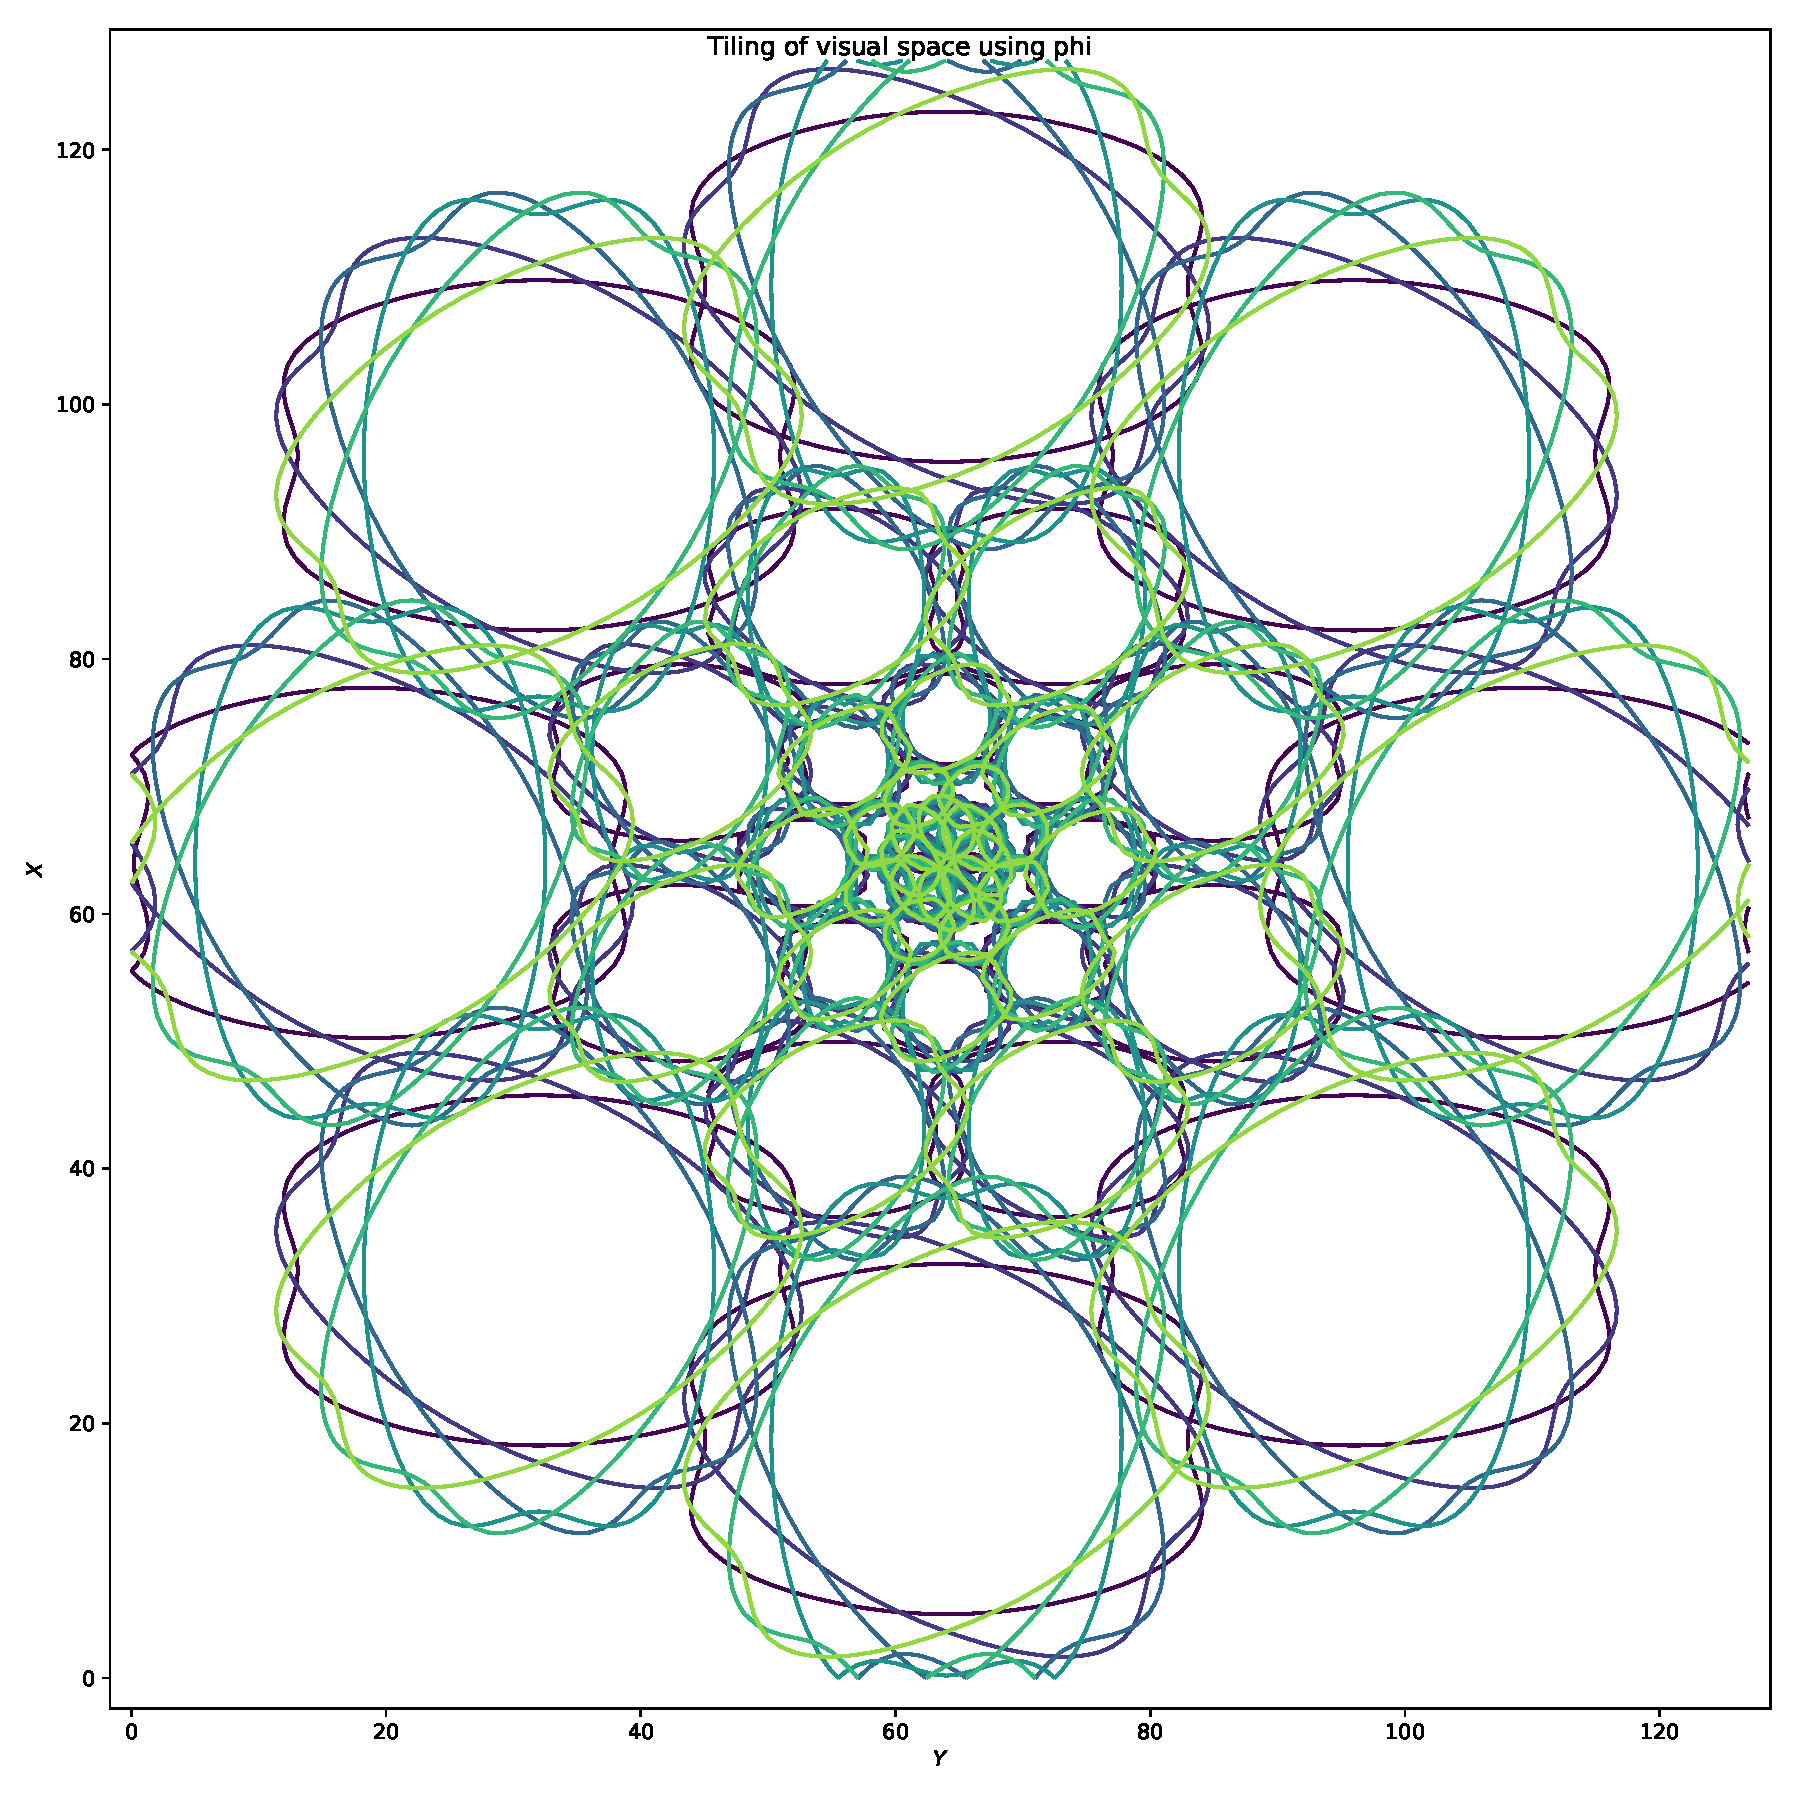
\includegraphics[scale=0.35]{Figures/LogPolar_shape}
\decoRule %puts an aesthetic horizontal line below the image
\caption[Figure]{Représentation graphique du filtre \textit{LogPolar} ($N_{theta}=6$,$N_{orient}=8$,$N_{scale}=5$,$N_{phase}=2$) }
\label{fig:LogPolar_shape}
\end{figure}

\begin{figure}[th]
\centering
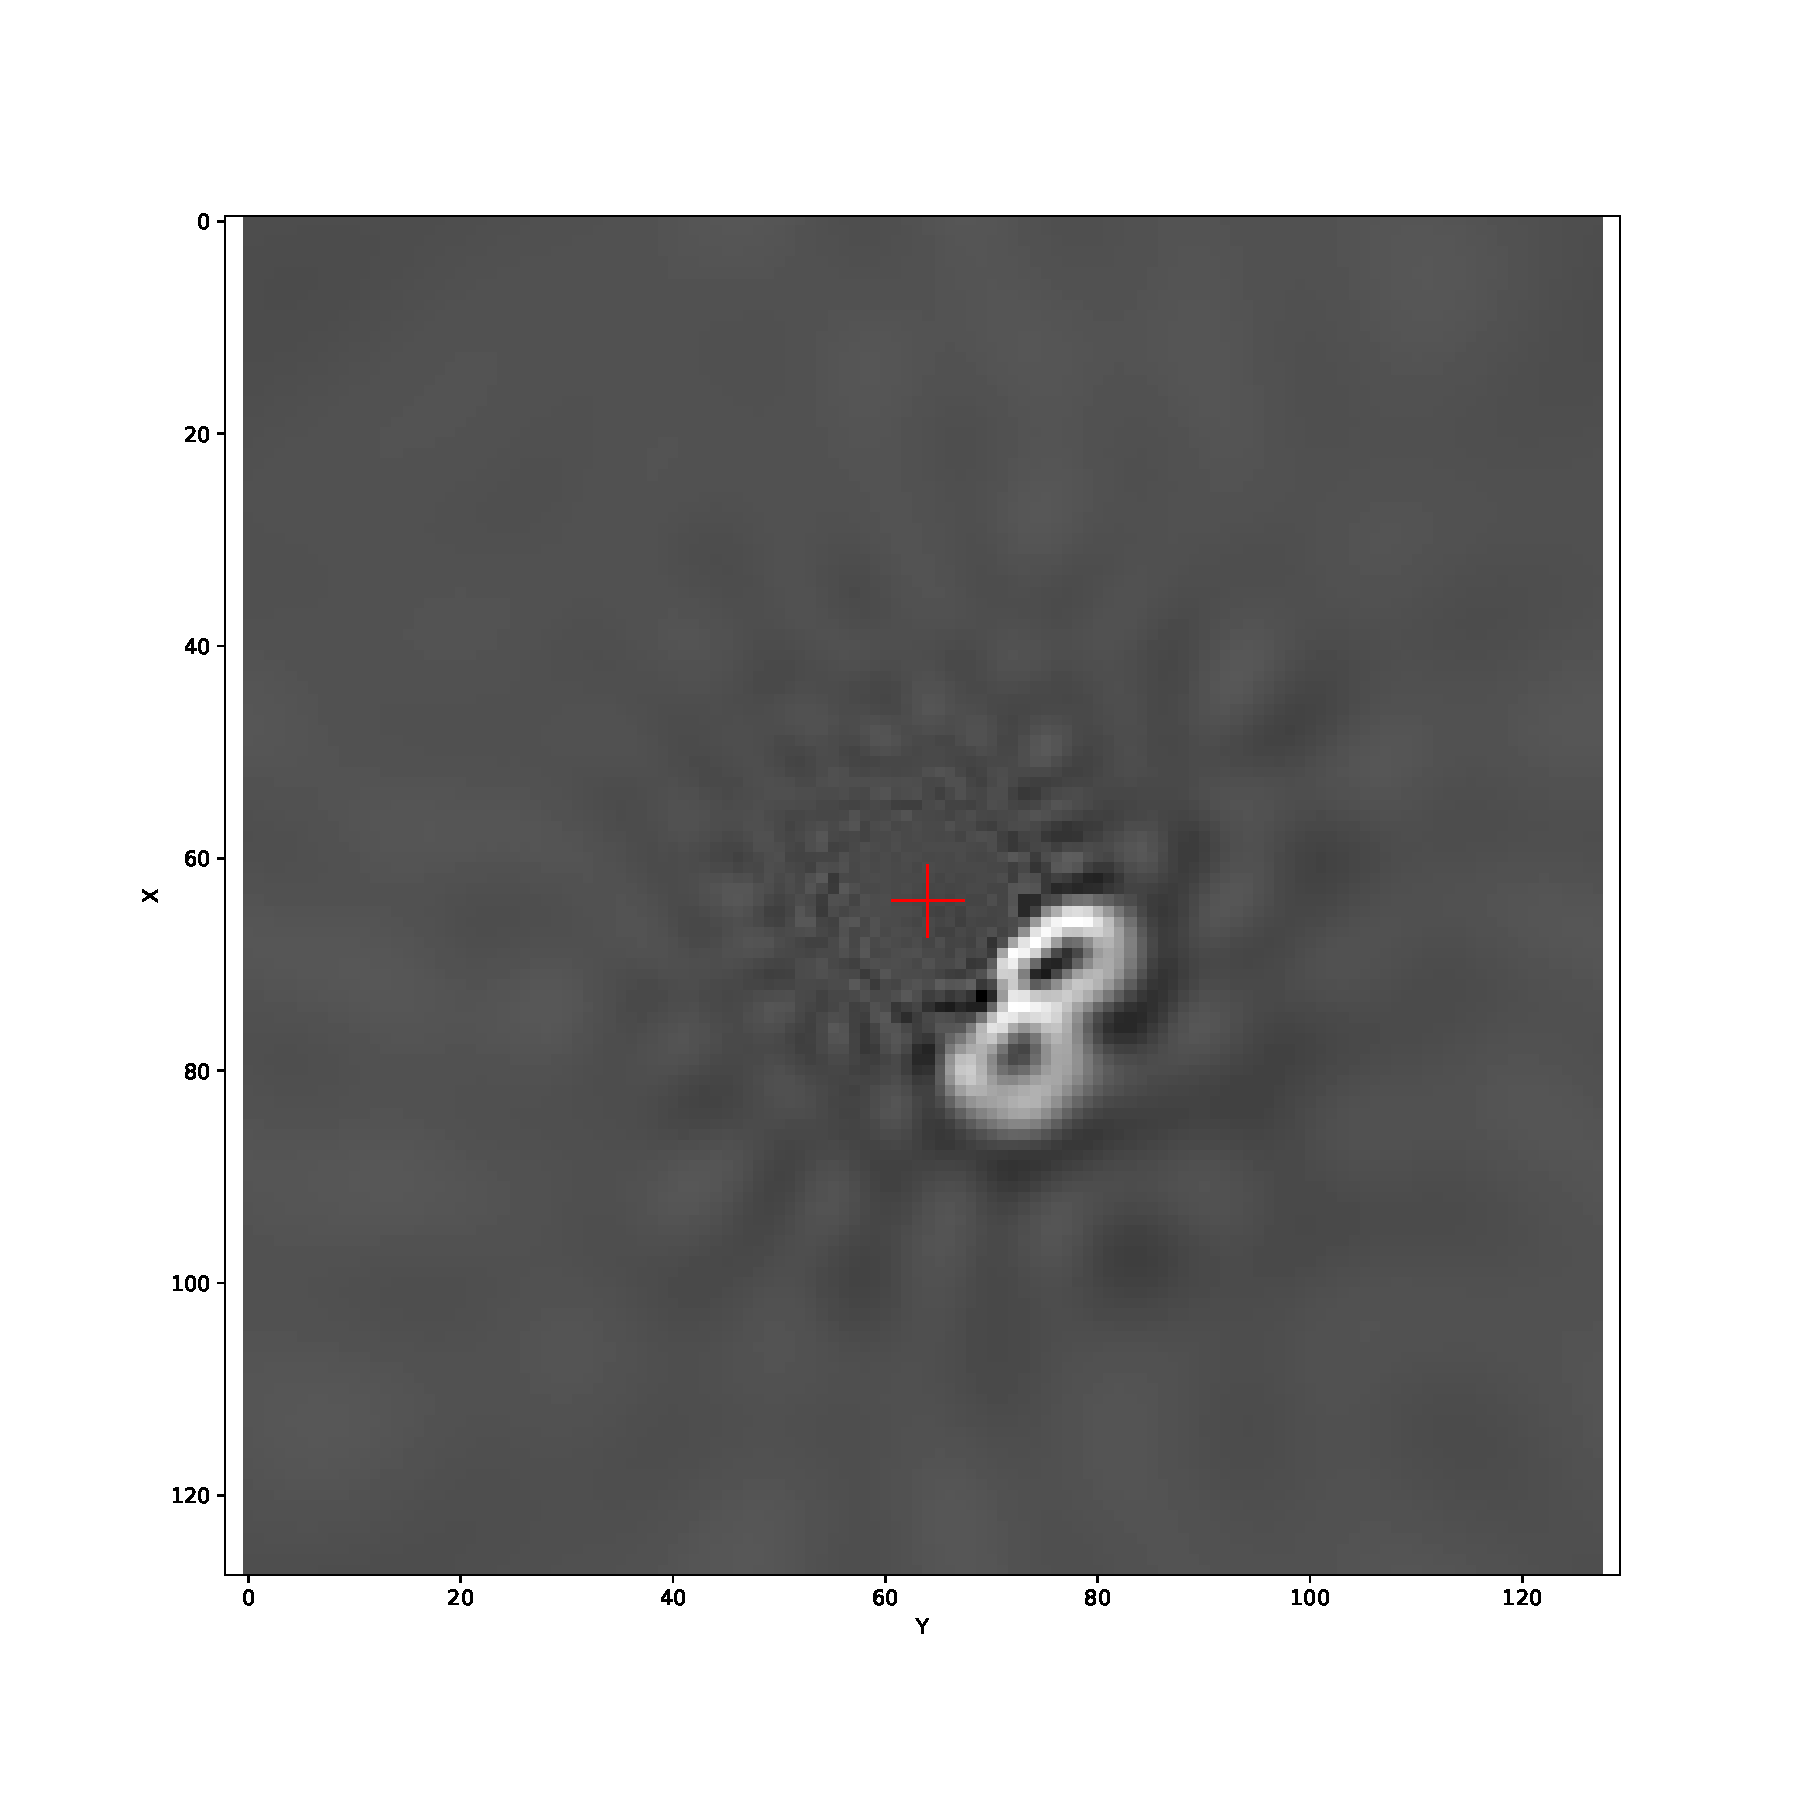
\includegraphics[scale=0.35]{Figures/LogPolar_effect}
\decoRule %puts an aesthetic horizontal line below the image
\caption[Figure]{Image après transformation par le filtre \textit{LogPolar} ($N_{theta}=6$,$N_{orient}=8$,$N_{scale}=5$,$N_{phase}=2$) }
\label{fig:LogPolar_effect}
\end{figure}

%%%%% Résultats %%%%%

\begin{figure}[th]
\centering
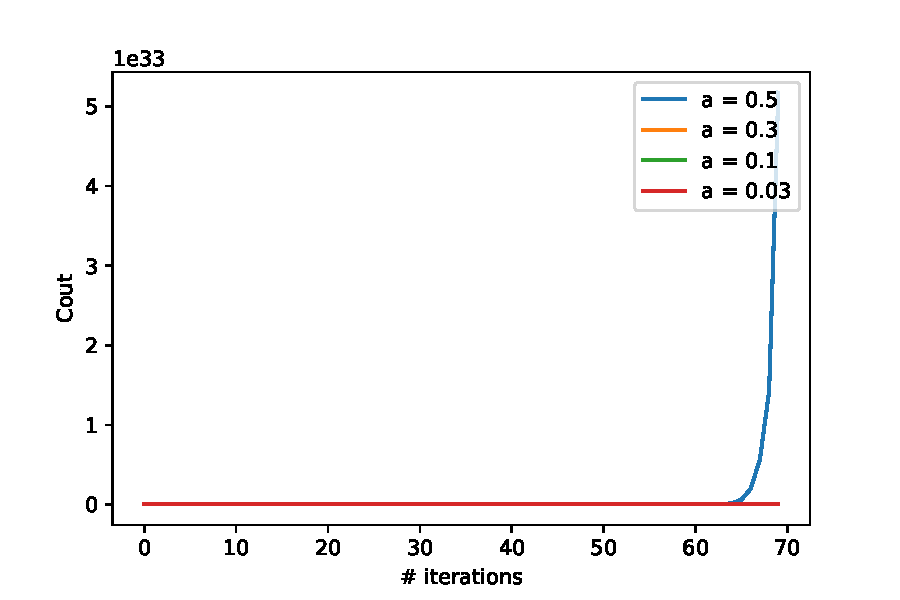
\includegraphics{Figures/Benchmarking_para_alpha_2}
\decoRule %puts an aesthetic horizontal line below the image
\caption[Figure]{Effet du paramètre alpha sur l'apprentissage dans le cadre d'un filtre \textit{Wavelets}}
\label{fig:benchmark_surApp1}
\end{figure}

\begin{figure}[th]
\centering
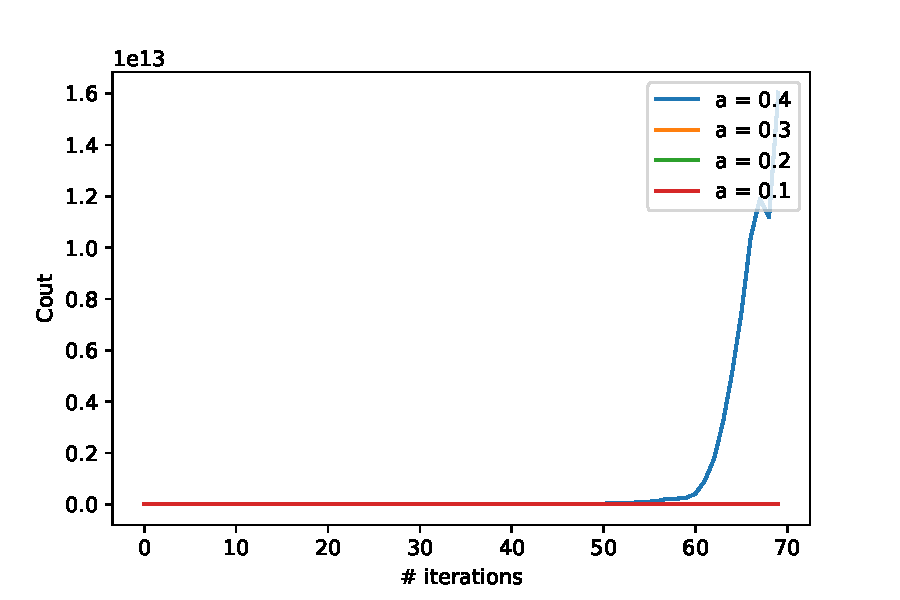
\includegraphics{Figures/Benchmarking_para_alpha_3}
\decoRule %puts an aesthetic horizontal line below the image
\caption[Figure]{Effet du paramètre alpha sur l'apprentissage dans le cadre d'un filtre \textit{Wavelets}}
\label{fig:benchmark_surApp2}
\end{figure}

\begin{figure}[th]
\centering
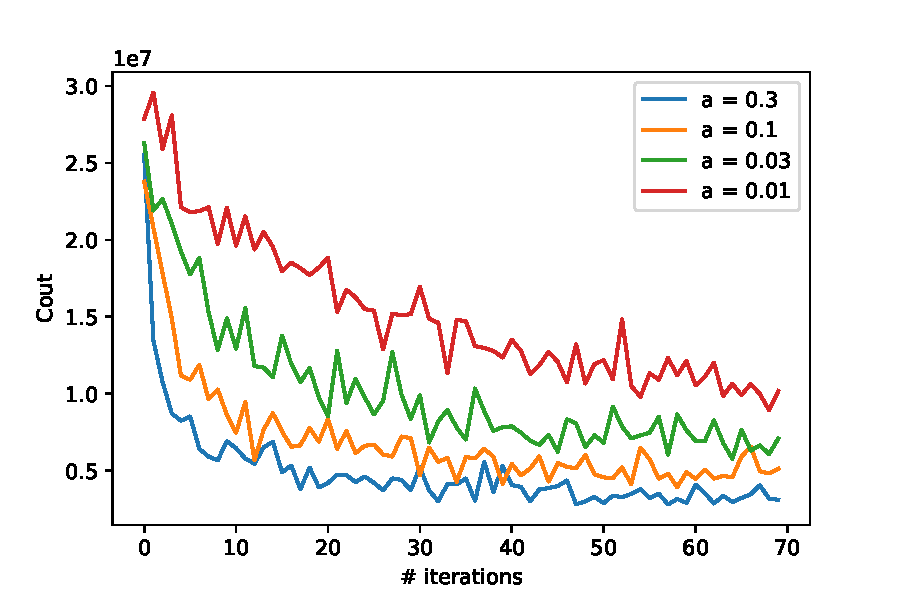
\includegraphics{Figures/Benchmarking_para_alpha}
\decoRule %puts an aesthetic horizontal line below the image
\caption[Figure]{Effet du paramètre alpha sur l'apprentissage dans le cadre d'un filtre \textit{Wavelets}}
\label{fig:benchmark_alpha}
\end{figure}

\begin{figure}[th]
\centering
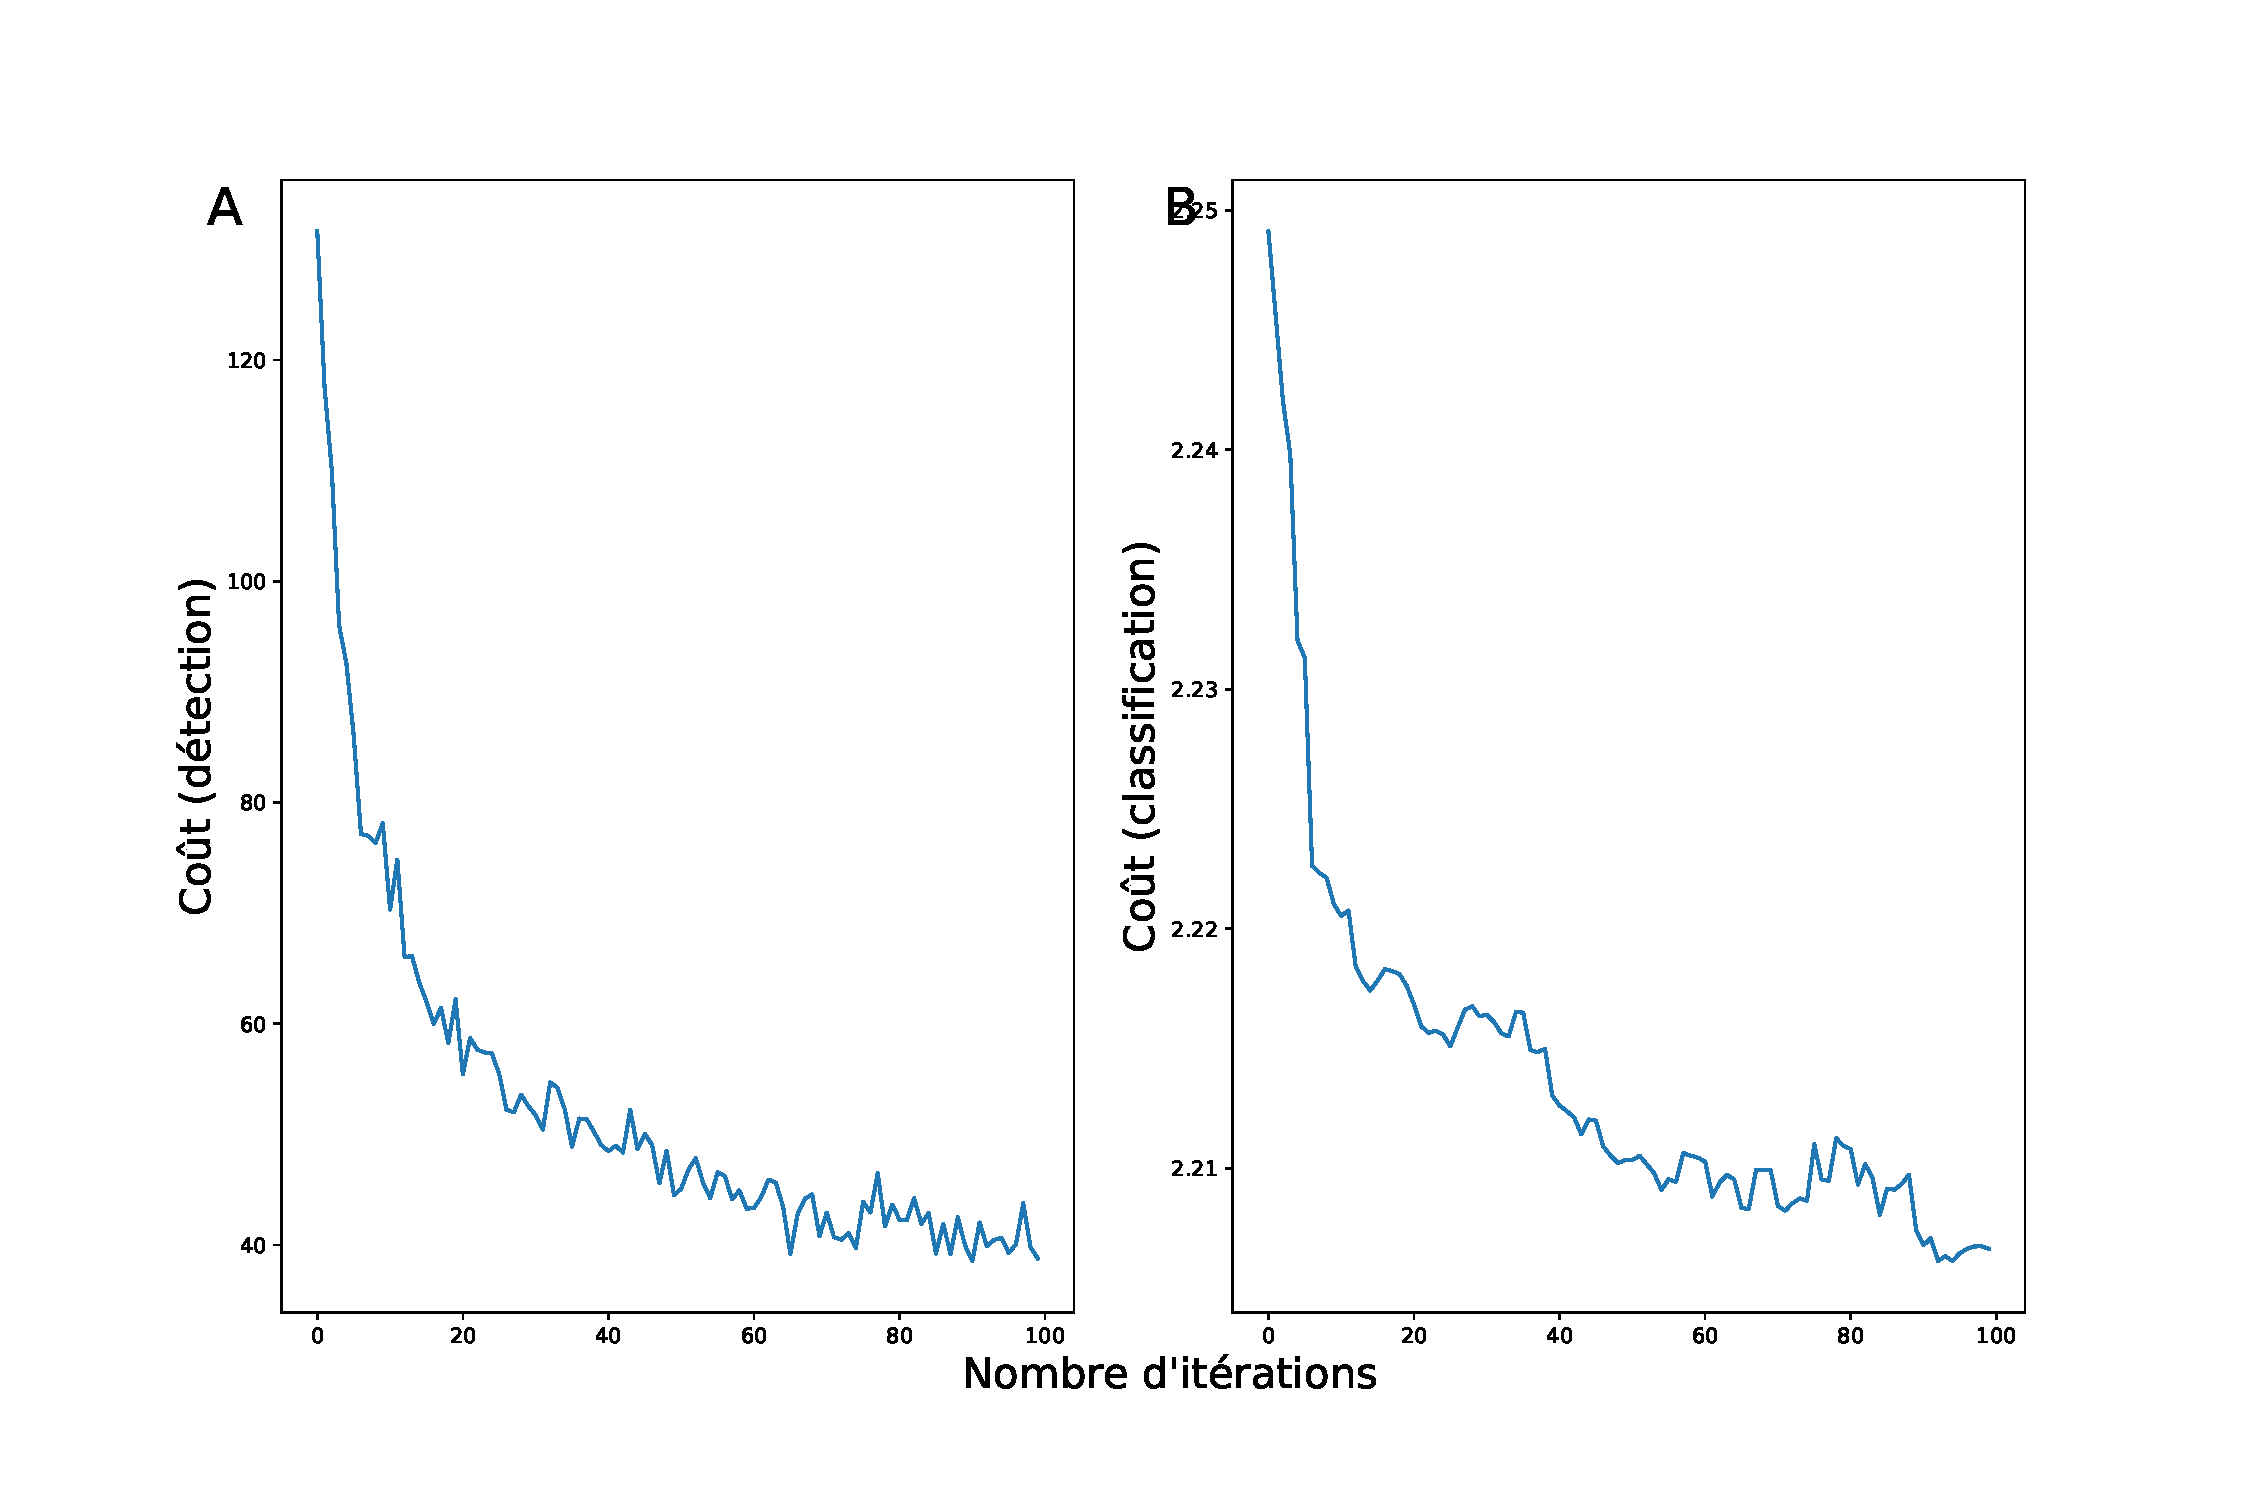
\includegraphics[scale=0.4]{Figures/logpolar_cost_learning}
\decoRule %puts an aesthetic horizontal line below the image
\caption[Figure]{Réduction du coût des couches \textit{détecteur} et \textit{classifieur} lors de l'apprentissage, dans le cadre d'un filtre \textit{LogPolar} (taille de la base d'apprentissage :  1000, nombre d'itérations : 100, $\alpha_{detect}=0.0015$, $\alpha_{classif}=0.3$)}
\label{fig:logpolar_cost}
\end{figure}

\begin{figure}[th]
\centering
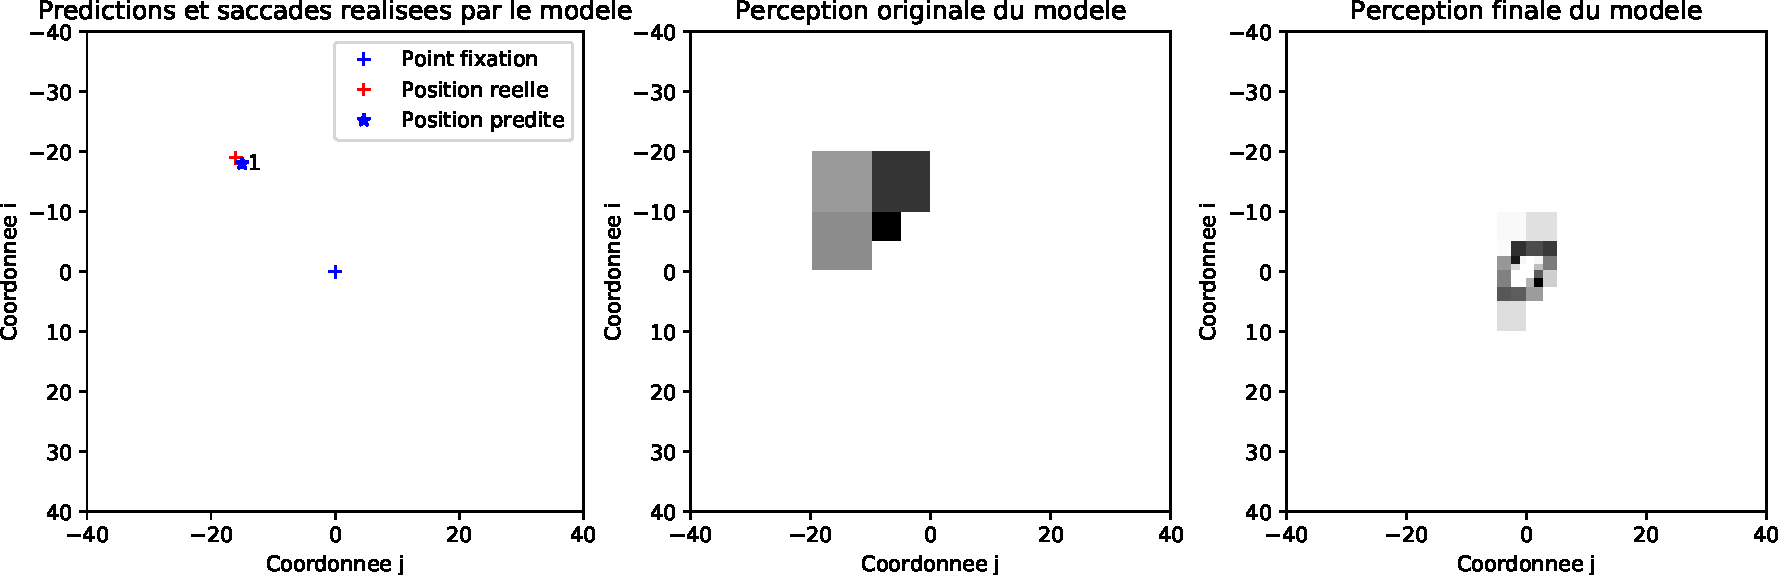
\includegraphics[scale=0.5]{Figures/saccades}
\decoRule %puts an aesthetic horizontal line below the image
\caption[Figure]{Perception et comportement saccadique du modèle entraîné, dans le cadre d'un filtre \textit{Wavelets}}
\label{fig:saccades}
\end{figure}

\begin{figure}[th]
\centering
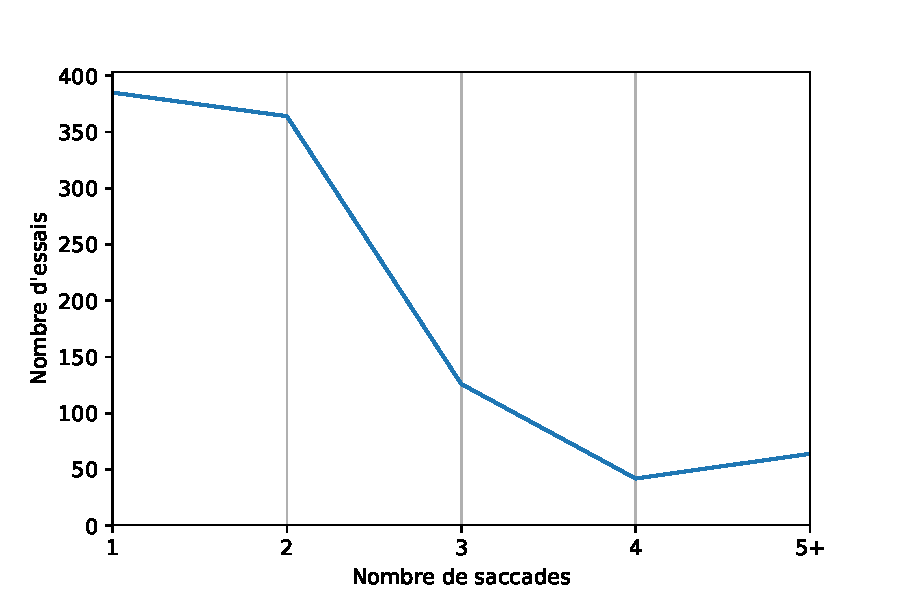
\includegraphics{Figures/sacc_nombre}
\decoRule %puts an aesthetic horizontal line below the image
\caption[Figure]{Nombre de saccades nécessaires pour atteindre la position de la cible au cours de 1000 essais, dans le cadre d'un filtre \textit{LogPolar} (taille de la base d'apprentissage :  1000, nombre d'itérations : 100, $\alpha_{detect}=0.0015$, $\alpha_{classif}=0.3$)}
\label{fig:sacc_nombre}
\end{figure}

\begin{figure}[th]
\centering
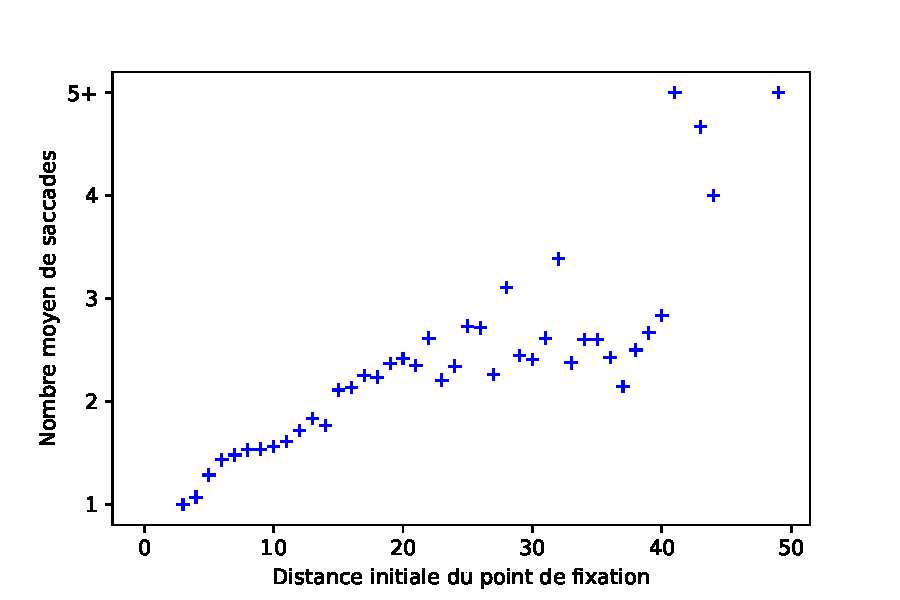
\includegraphics{Figures/sacc_distance}
\decoRule %puts an aesthetic horizontal line below the image
\caption[Figure]{Nombre moyen de saccades nécessaires pour atteindre la position de la cible en fonction de sa distance initiale du point de fixation au cours de 1000 essais, dans le cadre d'un filtre \textit{LogPolar} (taille de la base d'apprentissage :  1000, nombre d'itérations : 100, $\alpha_{detect}=0.0015$, $\alpha_{classif}=0.3$)}
\label{fig:sacc_distance}
\end{figure}

\begin{figure}[th]
\centering
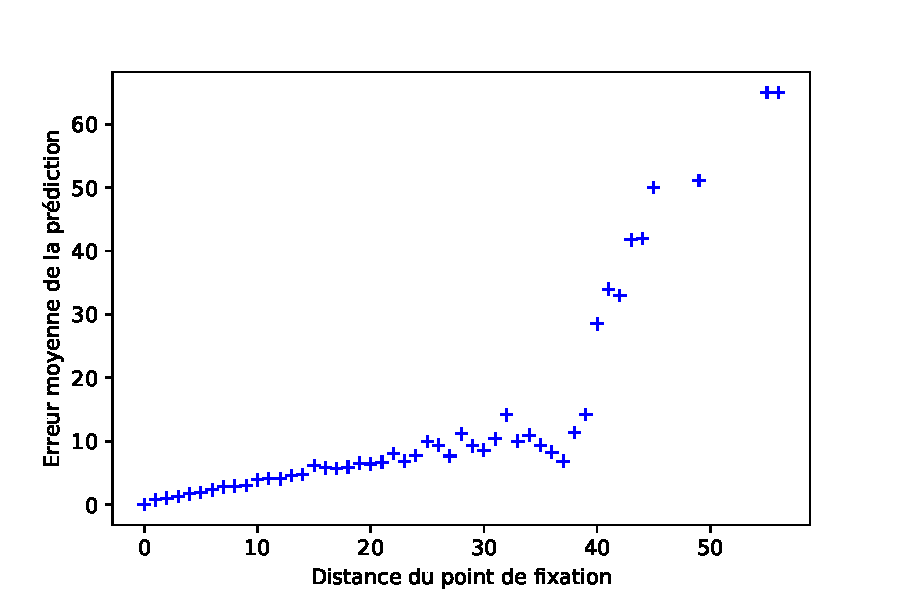
\includegraphics[scale=0.95]{Figures/err_distance}
\decoRule %puts an aesthetic horizontal line below the image
\caption[Figure]{Erreur moyenne lors de la prédiction de la position de la cible en fonction de sa distance du point de fixation au cours de 1000 essais, dans le cadre d'un filtre \textit{LogPolar} (taille de la base d'apprentissage :  1000, nombre d'itérations : 100, $\alpha_{detect}=0.0015$, $\alpha_{classif}=0.3$)}
\label{fig:err_distance}
\end{figure}